\section{Theory}

\subsection{Background}

\begin{frame}
    \frametitle{Markov Decision Process (MDP)}
    
    Framework for modeling decision making in partly random processes.\\
    In our case, \textit{partially observable} MDP~\cite{kaelbling_pomdp_1998}:

    \begin{itemize}
        \item \textit{Agent} interacts with \textit{environment} over discrete time steps \(t = 0, 1, 2\dots, T\).
        \item Takes \textit{action} \(a_t\) in state \(s_t\).
        \item Perceives (partial) \textit{observation} of state \(o_t\).
        \item New state \(s_{t+1}\) depends only on history of interactions.
        \item Agent must maintain some internal state depending on history \\
        \(\rightarrow\) memory needed!
    \end{itemize}

    \begin{figure}
        \centering
        \scalebox{0.75}{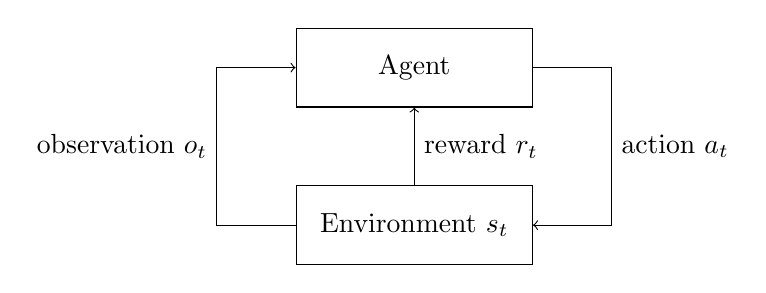
\begin{tikzpicture}[node distance=2cm]
    \tikzstyle{block} = [rectangle,minimum width=3cm,minimum height=1cm,text centered,draw=black,fill=white]
    \node (agent)[block]{Agent};
    \node (environment)[block,below of=agent]{Environment \(s_t\)};
    \draw [->] (agent.east) -- ++(1cm,0) -- node [anchor=west]{action \(a_t\)} ++(0,-2cm) -- (environment.east);
    \draw [->] (environment.north) -- node [anchor=west]{reward \(r_t\)} (agent.south);
    \draw [->] (environment.west) -- ++(-1cm,0) -- node [anchor=east]{observation \(o_t\)} ++(0,+2cm) -- (agent.west);
\end{tikzpicture}}
    \end{figure}
\end{frame}

\begin{frame}
    \frametitle{Reinforcement Learning (RL)}

    Paradigm for learning from interactions how to achieve a goal.

    \begin{itemize}
        \item Tasks usually formalized as (partially observable) MDPs.
        \item Policy \(\pi(a|s)\) is a mapping from states to actions.
        \item Find \(\pi\) that maximizes cumulative reward \(\mathbb{E} \left\lbrack \sum_{k=0}^{T} r_k \right\rbrack\).
        \item Often involves estimating the value \(v_\pi(s)\) of a state under policy \(pi\) (useful for training). 
    \end{itemize}

    Deep RL: Approximate \(\pi\) (and \(v_\pi\)) with deep neural networks.
    Has been used to play Atari~\cite{mnih_human_2015}, Go~\cite{silver_alphago_2016}, StarCraft II~\cite{vinyals_alphastar_2019}, etc.

\end{frame}

\subsection{Related Work}

\begin{frame}
    \frametitle{Search with Reinforcement Learning}

    \begin{itemize}
        \item Object localization (\cite{caicedo_active_2015,ghesu_artificial_2016,chen_memory_2017}).
        \item Visual navigation (\dots).
        \item Todo: add more related work.
    \end{itemize}
\end{frame}